\documentclass[resume]{subfiles}


\begin{document}
\begin{multicols}{3}
\section{PCB}
\subsection{Général}
Circuit haute vitesse : $t_r < 2\tau$ avec $t_r$ le temps de montée / descente et $\tau$ le temps de propagation ($L > \lambda/2$)
$$\tau=\frac{L}{\nu_{ph}}$$
Avec $\nu_{ph}$ la vitesse de propagation (typiquement $0.5$...$0.6c$)
$$\nu_{ph}=\frac{c}{\sqrt{\epsilon_r\mu_r}}$$
\paragraph{Extérieur} : Câbles, connecteurs, composants plus grands que $\lambda/10$
\paragraph{Sources de bruit} : PWM, bruit GND, oscillateurs, RF, spurious signals
\paragraph{Mesures de protection} : ferrites, filtres, opto-coupleurs, chokes, fibres optiques, R / L en série, shields, condensateurs, ferites au dela de \SI{100}{\mega\hertz}
\subsection{Guides d'ondes}
$$a=\frac{\lambda_c}{2}\qquad \lambda_c=\frac{c}{f_c}$$
$f_c$ la fréquence de transmission. Atténuation faible au delà et faible avant. Stitching $<\lambda/2$ pour éviter l'entrée / sortie d'ondes dans le pcb.\\
Transformation d'un guide d'onde en câble coax lorsqu'on place un conducteur interne
\subsection{Shielding}
Matériau du blindage, résonances, nombres de points de contact avec le plan GND
\subsection{Connecteurs}
\begin{figure}[H]
\centering
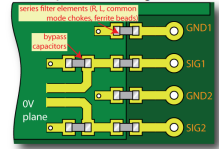
\includegraphics[width=4.00cm]{img_0.png}
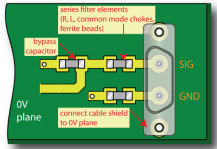
\includegraphics[width=4.00cm]{img_1.png}
\caption{Câble non-blindé vs câble blindé}
\end{figure}
\subsection{Filtrage}
\begin{figure}[H]
\centering
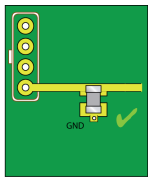
\includegraphics[width=2.00cm]{img_2.png}
\end{figure}
\subsection{Courant}
Chemin de retour du courant sur le plan le plus proche du signal (distribution gaussienne centrée sur la piste du signal). Si plusieurs chemins ou trop d'écartement $\longrightarrow$ tension/courant en mode commun et/ou bruit GND.\\
Possibilité de réduire le bruit en plaçant un plan (GND ou VCC) qui va servir de retour (plan image).\\
Les signaux différentiels produisent moins de perturbations et sont moins perturbés
\paragraph{Causes de courant en mode commun}
\begin{enumerate}
\item Retour par un plan de masse de section faible
\item Capacités différentes sur paires différentielles
\item Sources externes
\item Impédances différentes sur l'aller et le retour
\end{enumerate}

\subsection{Pistes}
\begin{figure}[H]
\centering
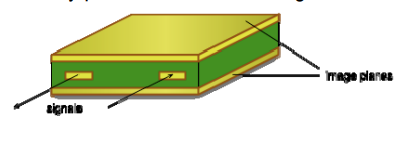
\includegraphics[width=4.00cm]{img_3.png}
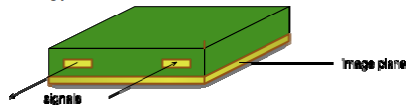
\includegraphics[width=4.00cm]{img_4.png}
\caption{Stripline vs Microstrip}
\end{figure}
\paragraph{Méthodologie}
\begin{enumerate}
\item Définition des couches
\item Placer les connecteurs et les vis
\item Placer les composants critiques
\item Zones du PCB (numérique, analogique)
\item Layout
\end{enumerate}
\subsection{Couches}
\begin{enumerate}
\item S-G-V-S (économie de vias, bonne protection)
\item S-G-S-B (pas symétrique, très bonne protection)
\item G-S-S-V (beaucoup de vias, trous dans les plans)
\end{enumerate}
\subsubsection{Empilements à utiliser}
\begin{enumerate}
\item S-G-V-S
\item S-G-S--S-V-S
\item S-G-V-S-S-V-G-S
\end{enumerate}
\subsection{Plan de masse}
\paragraph{Masse chaude} : fait le tour du circuit (vis, connecteurs)
\paragraph{Masse froide} : GND interne du circuit
Les deux masses sont reliées par un pont qui empêche le passage des perturbations.\\
Il faut éviter les interruptions du plan de masse (surtout si elles sont longues).\\
Lorsqu'il y a plusieurs plans de masse (AGND, DGND), on utilise une connexion en étoile.\\
Remplir toutes les zones non-utilisées par des plans de masse (ou de VCC)
\subsubsection{Séparation du plan de masse}
\begin{multicols}{2}
\begin{enumerate}[label={+}]
\item isolation de zones
\item Contrôle des chemin de retour 
\item Réduction des capacités parasites
\end{enumerate}
\begin{enumerate}[label={-}]
\item Les coupures peuvent générer des antennes
\item Pas forcément utile
\end{enumerate}
\end{multicols}

\subsection{Antennes}
Champ électrique $E$ généré par une boucle d'aire $A$ traversée par un courant $I$ à une distance $R$
$$E\sim \frac{k^2 IA}{4\pi}\sqrt{\frac{\mu}{\epsilon}}\left(\frac{1}{R}\right)\qquad k=\frac{2\pi}{\lambda}=\frac{\omega}{c}$$
\subsubsection{Antenne dipôle}
\begin{figure}[H]
\centering
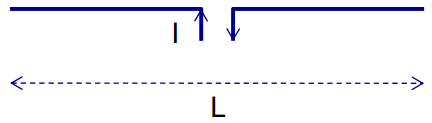
\includegraphics[width=3.00cm]{img_5.png}
\end{figure}
$$E\sim \frac{ILf}{4\epsilon_0 R}$$
\subsubsection{Antenne "slot"}
\begin{figure}[H]
\centering
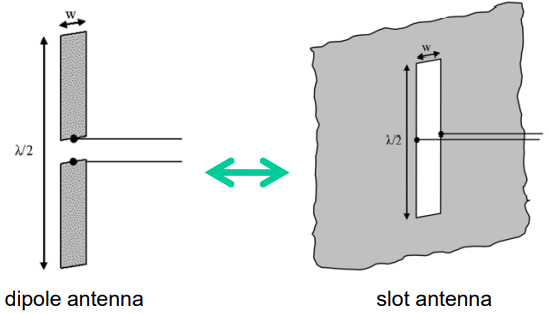
\includegraphics[width=5.00cm]{img_6.png}
\end{figure}
$$f=\frac{c}{\lambda}$$
\subsection{Horloge}
Rapport signal sur bruit dû au jitter :
$$\text{SNR}=20\log_{10}\left(\frac{1}{2\pi ft_\text{jitter}}\right)$$


\end{multicols}
\end{document}